\section{Experiments and results}\label{sec:chp6:exp-res}

In this section, different experiments are proposed to design and investigate our \ac{mpmri} \ac{cad} for the detection of \ac{cap}.
First, the classification performance of each independent modality is investigated in \acs{sec}\,\ref{subec:chp6:exp-res:Ex1}.
For each modality, the ``quantification'' approaches maximizing the classification performance are selected.
Additionally, we attend to directly combined \ac{mpmri} modalities, which we referred as ``coarse'' combination as presented in \acs*{sec}\,\ref{subsec:chp6:exp-res:Ex2}.
Subsequently, \acs{sec}\,\ref{subsec:chp6:exp-res:Ex3} presents the benefit of balancing the dataset on the learning stage and strategies for feature selection and extraction, for each feature modality as well as an aggregation of them.
Consequently, different combination classifier rules are studied using the previous fine-tuned feature space in \acs{sec}\,\ref{subsec:chp6:exp-res:Ex4}.
Finally, we conclude in \acs{sec}\,\ref{subsec:chp6:exp-res:Ex5} by investigating the benefit of fusing the \ac{mrsi} information with the other modality.

All these experiments are conducted on a subset of the public \ac{mpmri} prostate presented in \acs{sec}\,\ref{sec:data3t}.
We used the \SI{3}{\tesla} dataset which is composed of a total of 20 patients of which 18 patients had biopsy proven \ac{cap} and 2 patients are ``healthy'' with negative biopsies. 
In this study, our subset consists of 17 patients with \ac{cap}.

\subsection{Assessment of classification performance of individual modality}\label{subec:chp6:exp-res:Ex1}

In this experiment, we attend to assess the classification performance of each individual \ac{mri} modality.

\paragraph{\ac{t2w}-\ac{mri} and \ac{adc} map features} All features presented in \acs{tab}~\ref{tab:featureadct2w} are extracted for both \ac{t2w}-\ac{mri} and \ac{adc} map.
These features are combined per modality and for each of them, a \ac{rf} classifier is trained.

\begin{landscape}
\begin{figure}
  \hspace*{\fill}
  \subfigure[Performance of the quantitative methods on \acs*{dce}-\acs*{mri}.]{\label{fig:inddcemodel}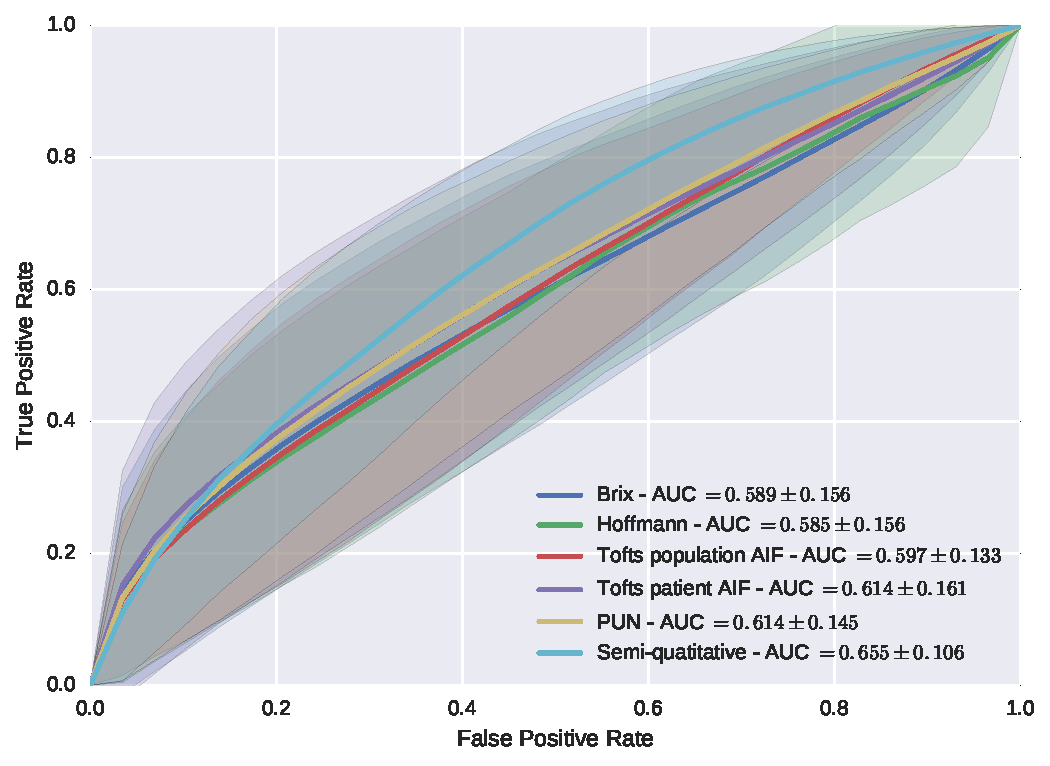
\includegraphics[height=.4\textheight]{5_normalization/figures/DCE-normalization/normalized_methods_0.pdf}}
  \hfill
  \subfigure[Performance of enhanced \acs*{dce}-\acs*{mri} signal.]{\label{fig:inddcesignal}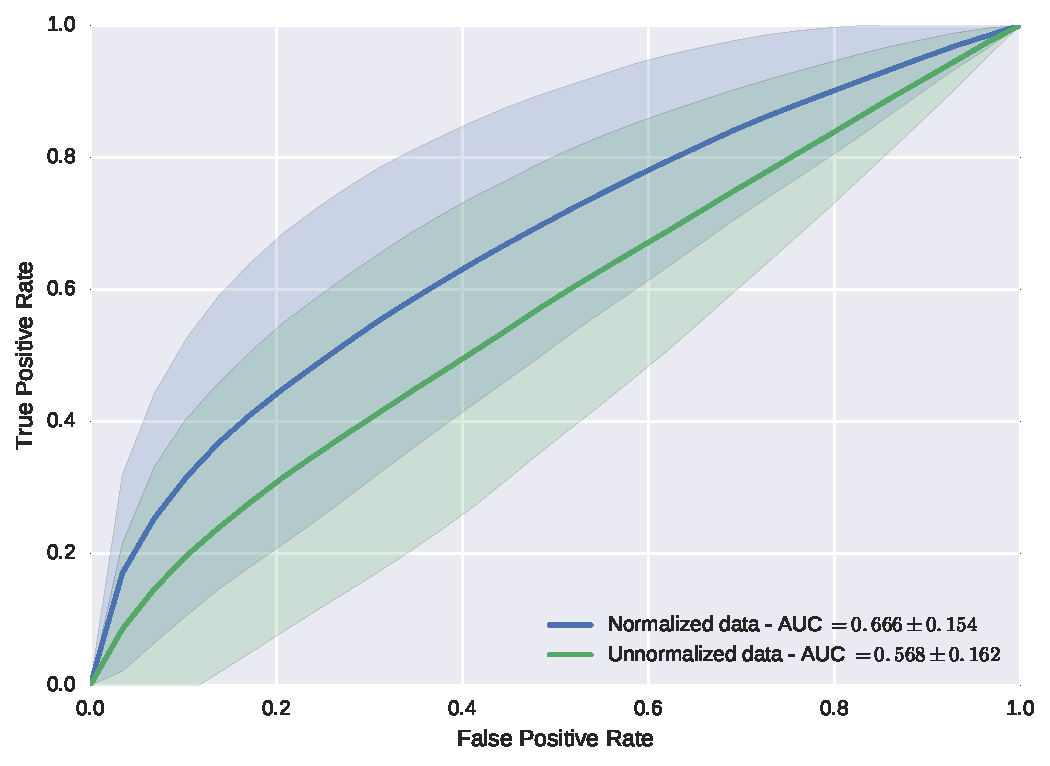
\includegraphics[height=.4\textheight]{5_normalization/figures/DCE-normalization/full_signal_0.pdf}}
  \hspace*{\fill} \\
  \hspace*{\fill}
  \subfigure[Performance of image-based features for \acs*{t2w}-\acs*{mri} and \acs*{adc} map.]{\label{fig:indadct2w}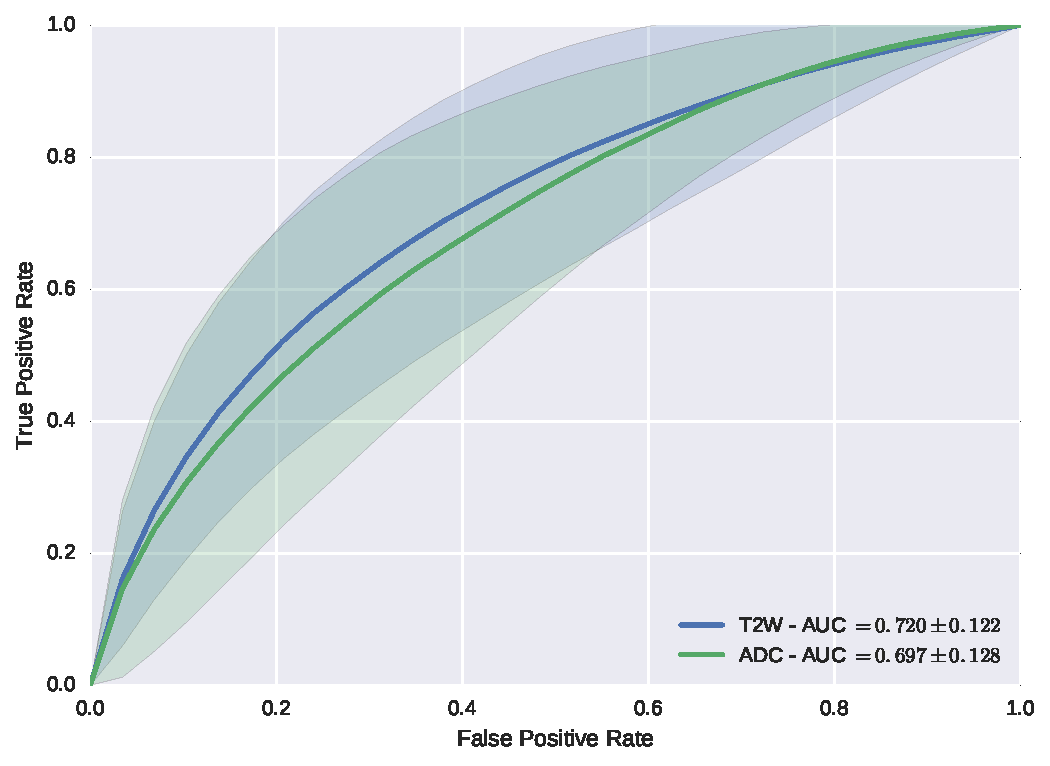
\includegraphics[height=.4\textheight]{6_pipeline/figures/exp-1/t2w_adc.pdf}}
  \hfill
  \subfigure[Performance of different approach for the \acs*{mrsi} modality.]{\label{fig:indmrsi}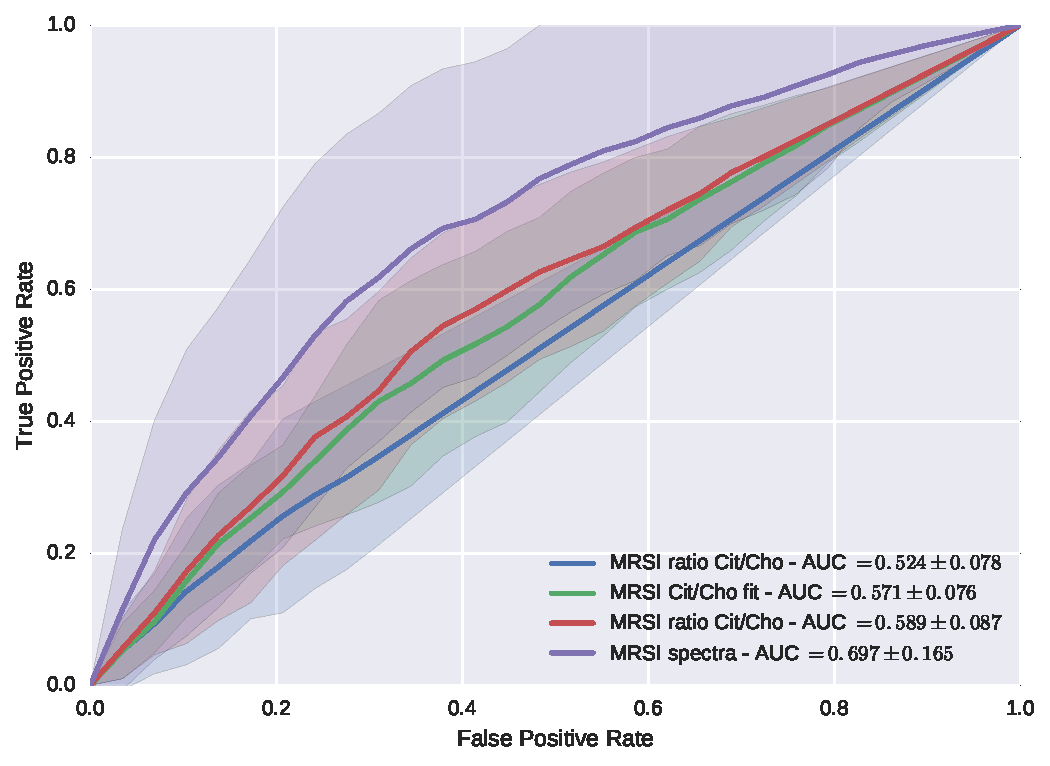
\includegraphics[height=.4\textheight]{6_pipeline/figures/exp-1/mrsi_all.pdf}}
  \hspace*{\fill}
  \caption[Analysis of the classification performance for each individual \acs*{mri} modality.]{Analysis of the classification performance for each individual \acs*{mri} modality. Different models have been tested for \acs*{dce}-\acs*{mri} and \acs*{mrsi} modalities.}
  \label{fig:res-Ex1}
\end{figure}
\end{landscape}


\paragraph{\ac{dce}-\ac{mri} features} This experiment has been presented in \acs{sec}\,\ref{subsec:chp5:DCE-norm:exp-res}.
We attend to find the most discriminative ``quantification'' method for \ac{dce}-\ac{mri} modality, by assessing the classification performance of the different models.
Therefore, the pharmacokinetic parameters from the Brix, Hoffmann, Tofts, and \ac{pun} models, the semi-quantitative parameters, and the enhanced \ac{dce}-\ac{mri} signal are extracted.
For each set of feature, a \ac{rf} classifier is trained.

\paragraph{\ac{mrsi} features} Similarly to \ac{dce}-\ac{mri}, 4 \ac{rf} classifiers are trained on different features:
(i) the cropped \ac{mrsi} signal,
(ii) the relative concentration of the citrate over the relative concentration of the choline, both computed through fitting as presented in the previous section,
(iii) the ratio of the two previous features, and finally
(iv) the ratio of the relative concentration of the citrate over the relative concentration of the choline, using fix integration bounds.

\paragraph{Results}
Each trained \ac{rf} is evaluated using a \ac{lopo}.
A \ac{roc} analysis is carried out and the \ac{auc} score is computed to report and compare the classification performance of each classifier.
The results are depicted in \acs{fig}\,\ref{fig:res-Ex1}.
As presented is the previous chapter, classification of \ac{dce}-\ac{mri} data using the normalized enhanced \ac{dce}-\ac{mri} signal is strategy leading the highest \ac{auc} --- i.e., $0.666 \pm 0.154$ ---, outperforming any quantification method.
Similarly these findings, classification of the cropped \ac{mrsi} signal outperforms other quantification-based methods, with an \ac{auc} of $0.697 \pm 0.165$.
Classification of the extracted features based on \ac{adc} offer an close performance with an identical mean \ac{auc} and a smaller standard deviation of $0.128$.
Finally, the features extracted from \ac{t2w}-\ac{mri} are shown to be the most discrimnative with an \ac{auc} reaching $0.720 \pm 0.122$.
As a conclusion, the most efficient features in term of classification performance for each modality are selected for the remainder of the experiment section.

\subsection{Coarse combination of \acs*{mpmri} modalities} \label{subsec:chp6:exp-res:Ex2}

\begin{figure}
  \centering
  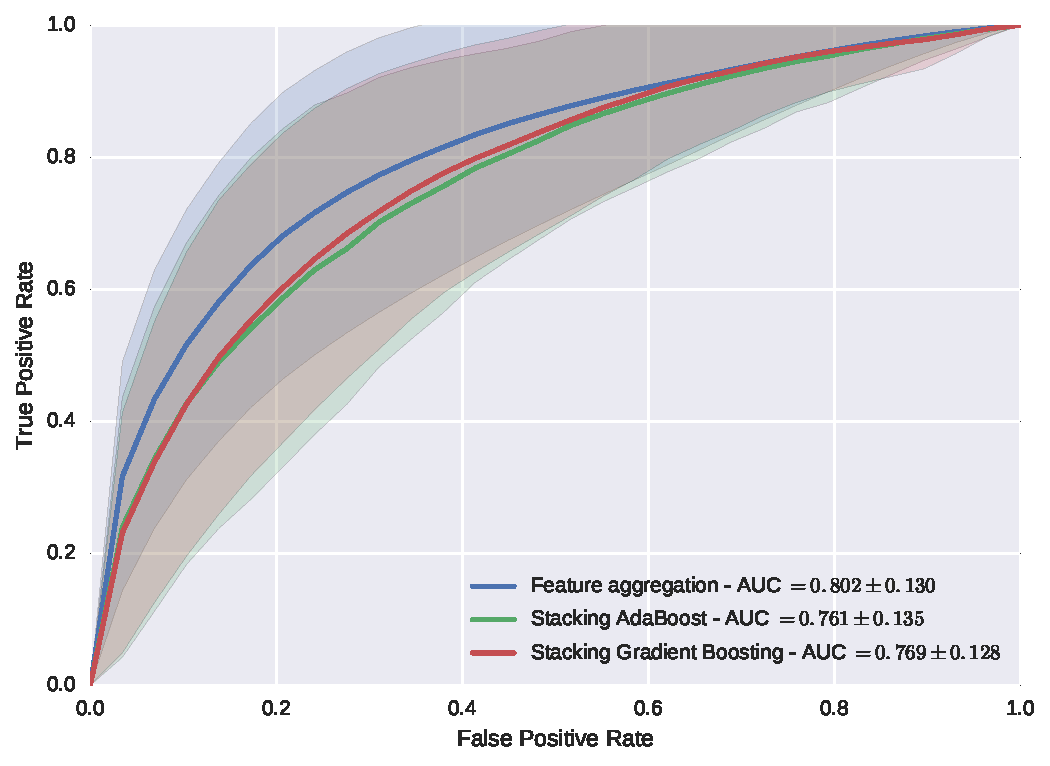
\includegraphics[width=0.7\linewidth]{6_pipeline/figures/exp-2/comb_all.pdf}
  \caption[Comparison of different combination approaches.]{Comparison of different combination approaches: (i) aggregation of the different features in conjunction with a \acs*{rf} classifier, (ii) a stacking approach using 4 \acs*{rf}s and \acs*{adb} as meta-classifier, and (iii) a stacking approach using 4 \acs*{rf}s and \acs*{gb} as meta-classifier.}
  \label{fig:res-Exp2}
\end{figure}

As a first attempt to design a \ac{mpmri} \ac{cad} system, 3 different approaches are used to combine the selected feature from each modality:
(i) feature aggregation,
(ii) stacking using \ac{adb},
(iii) stacking using \ac{gb}.
We refer these combinations as being coarse since no tuning --- i.e., feature balancing/selection/extraction --- aiming at improving the classification performance is involved.
This experiment can be considered as the baseline to obtain a \ac{mpmri} \ac{cad} for the detection of \ac{cap}.

In the first approach, the features from all the different modality are concatenated together to form a unique matrix.
Additionally, the anatomical features are concatenated within the same matrix.
The second and third approaches are based on the stacking which has been presented in the previous section.
They differ in the choice of the meta-learner since the first stack uses an \ac{adb} classifier while the second stack uses a \ac{gb}.
Each base learner is similar to the \ac{rf} selected in the previous experiment.
The difference lie in the concatenation of the anatomical features with each feature set derived from the \ac{mri} modality presented in the previous experiment.

\paragraph{Results}
The three coarse combinations are tested using a \ac{lopo}.
Furthermore, for the stacking approaches, the training set is split into a smaller training set and a validation set composed of 10 and 6 patients, respectively.
A \ac{roc} analysis is carried out for each combination and the \ac{auc} is computed as reported in \acs{fig}\,\ref{fig:res-Exp2}.

A single learner using aggregated features outperform the stacking-based classifier with an \ac{auc} of $0.802 \pm 0.130$.
Furthermore, \ac{gb} chosen as a meta-classifier lead to better classification performance than \ac{adb}, with an improved \ac{auc} from $0.761 \pm 0.135$ to $0.769 \pm 0.128$.

\subsection{Benefits of data balancing and feature selection/extraction}\label{subsec:chp6:exp-res:Ex3}

In this section, we attend to optimize the different feature set used in the previous classification.
Therefore, our contribution is twofold: (i) we compare the different balancing methods to distinguish which method is the best suited and (ii) feature selection/extraction methods are used to identify which feature are the most discriminative among each set.

\begin{figure}
  \centering
  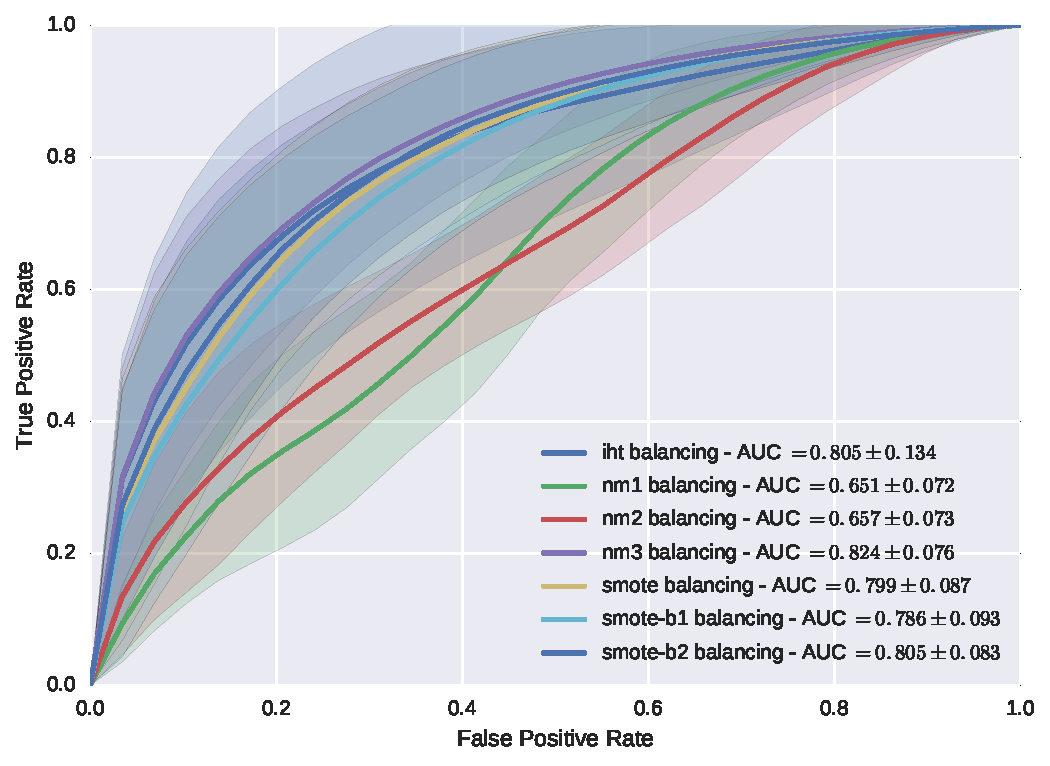
\includegraphics[width=0.7\linewidth]{6_pipeline/figures/exp-3/all.pdf}
  \caption{Analysis of the benefit of balancing the training dataset before the learning process while concatenating all features.}
  \label{fig:allbalance}
\end{figure}

\paragraph{Comparison of balancing strategies}
For this experiment, a \ac{rf} classifier is trained for each feature set selected from the first experiment.
As in the previous experiment, a \ac{lopo} is used as validation model.
During the learning phase, the training set are balanced using the methods presented in \acs{sec}\,\ref{subsec:chp6:method:fea-bal}.
The possible improvements offered by the balancing methods is analyzed through a \ac{roc} analysis and computing the \ac{auc}.
The results are depicted in \acs{fig}\,\ref{fig:res-Ex3-bal} and give rise to two observations:
(i) there is at least one balancing method which improves the classification performance and
(ii) \ac{iht} and \ac{smote} are the methods performing the best on individual modality features.
On the one hand, \ac{iht} outperforms the other methods while balancing the feature sets based on the \ac{dce}-\ac{mri} and \ac{adc} map.
The \ac{auc} increases of $0.019$ and $0.018$ for the feature sets of the \ac{dce}-\ac{mri} and \ac{adc} map, respectively.
On the other hand, \ac{smote} increases the \ac{auc} of $0.042$ for \ac{t2w}-\ac{mri}.
However, there is no significant improvement for the \ac{mrsi} since only the standard deviation of the \ac{auc} decreases of $0.019$.
Once all features are concatenated together, \ac{nm3} is the method providing the best enhancement of the classification performance with an \ac{auc} of $0.824 \pm 0.076$, as depicted in \acs{fig}\,\ref{fig:allbalance}.
In conclusion, the methods leading to the best performance are applied prior to feature selection/extraction for the remainder of the experiment.

\paragraph{Feature selection and extraction}

Noisy or non-discriminative features included in the learning process might degrade the overall performance of a classifier.
Thus, the feature selection and extraction methods presented in \acs{sec}\,\ref{subsec:chp6:method:fea-bal} are used to obtain a fine-tuned feature space.
The selection approaches --- i.e., \ac{anova} F-value and Gini importance --- are applied on the image-based features extracted from \ac{t2w}-\ac{mri} and \ac{adc} map modalities.
For both methods, a threshold defines the percentage of features to select.
Additionally, several thresholds are defined to find the number of features maximizing the classification performance.

Features computed from \ac{mrsi} and \ac{dce}-\ac{mri} modalities are related to signal and feature extraction seems more appropriate than feature selection rather than feature selection.
Therefore, the 3 feature extraction methods --- i.e., \ac{pca}, sparse-\ac{pca}, and \ac{ica} --- are applied by varying the number of components or the sparsity level, which allow to find the level which maximized the classification performance.
Finally, the feature selection methods have been applied on the concatenation of all the features.

As the previous experiments, the classification is performed using a \ac{rf} with \ac{lopo} model validation.
A \ac{roc} analysis is performed and for each \ac{roc}, the \ac{auc} score is computed.
The results are reported from \acs{tab}~\ref{tab:ginit2w} to \acs{tab}~\ref{tab:anovacomb}, in which the best results are highlighted in \textbf{bold}.

\begin{landscape}
\begin{figure}
  \hspace*{\fill}
  \subfigure[\ac{t2w}-\ac{mri}]{\label{fig:ex3:T2W}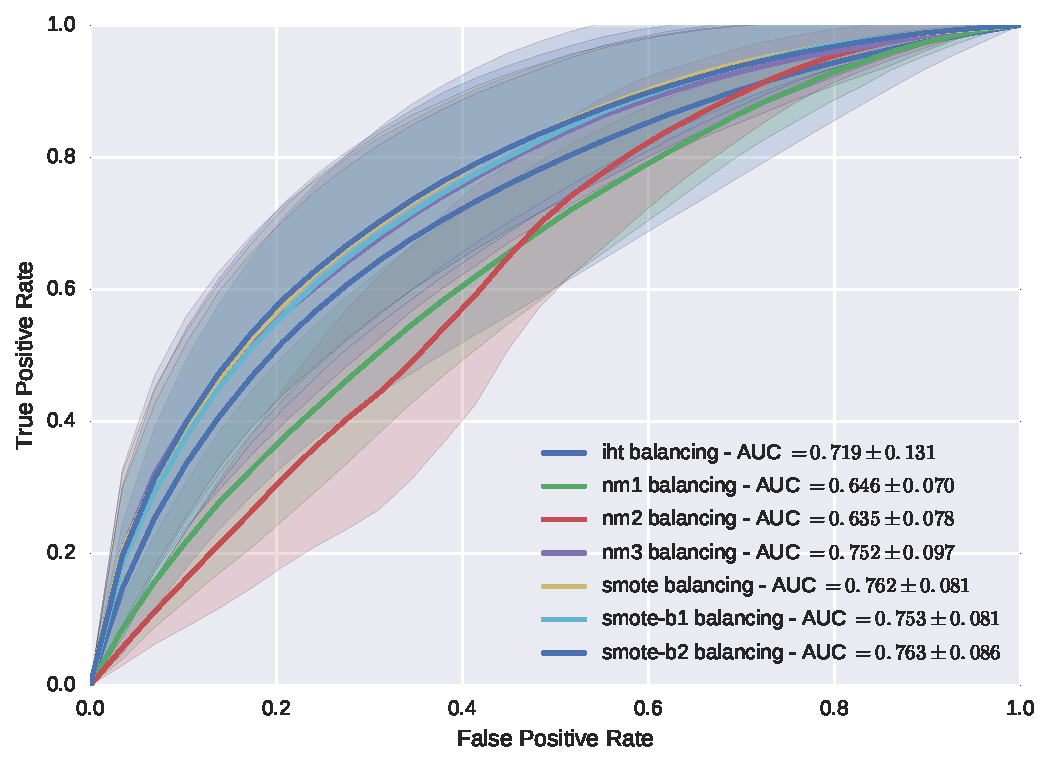
\includegraphics[height=.4\textheight]{6_pipeline/figures/exp-3/t2w.pdf}}
  \hfill
  \subfigure[\ac{adc}-\ac{mri}]{\label{fig:ex3:ADC}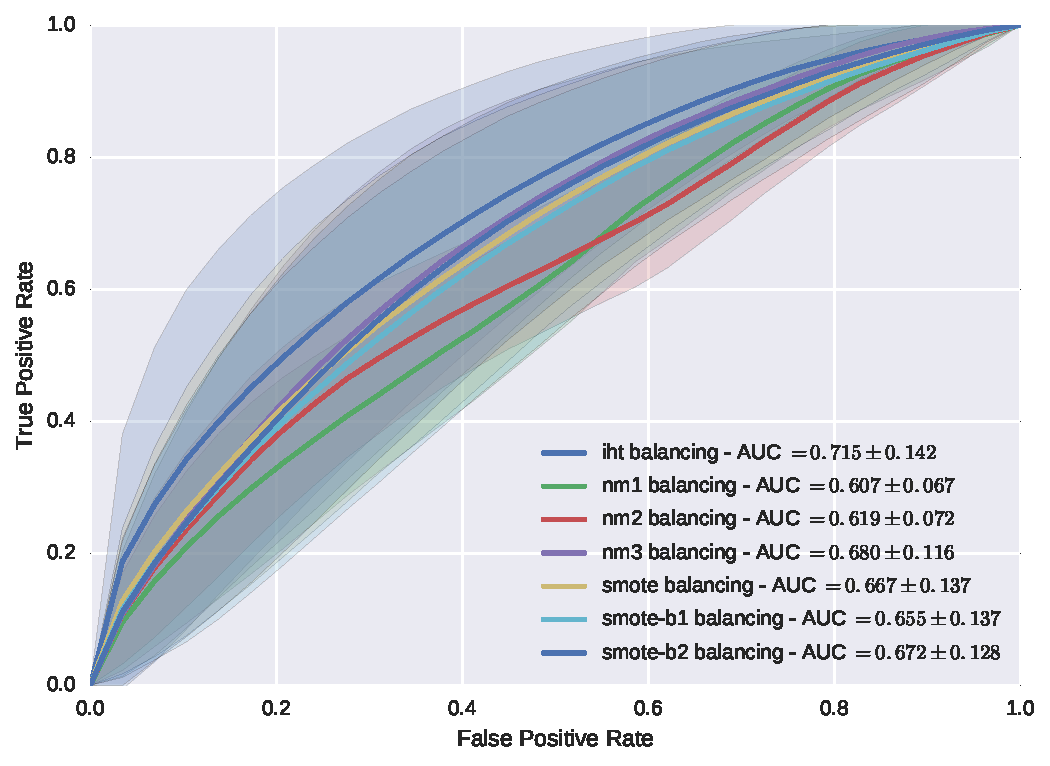
\includegraphics[height=.4\textheight]{6_pipeline/figures/exp-3/adc.pdf}}
  \hspace*{\fill} \\
  \hspace*{\fill}
  \subfigure[\ac{dce}-\ac{mri}]{\label{fig:ex3-DCE}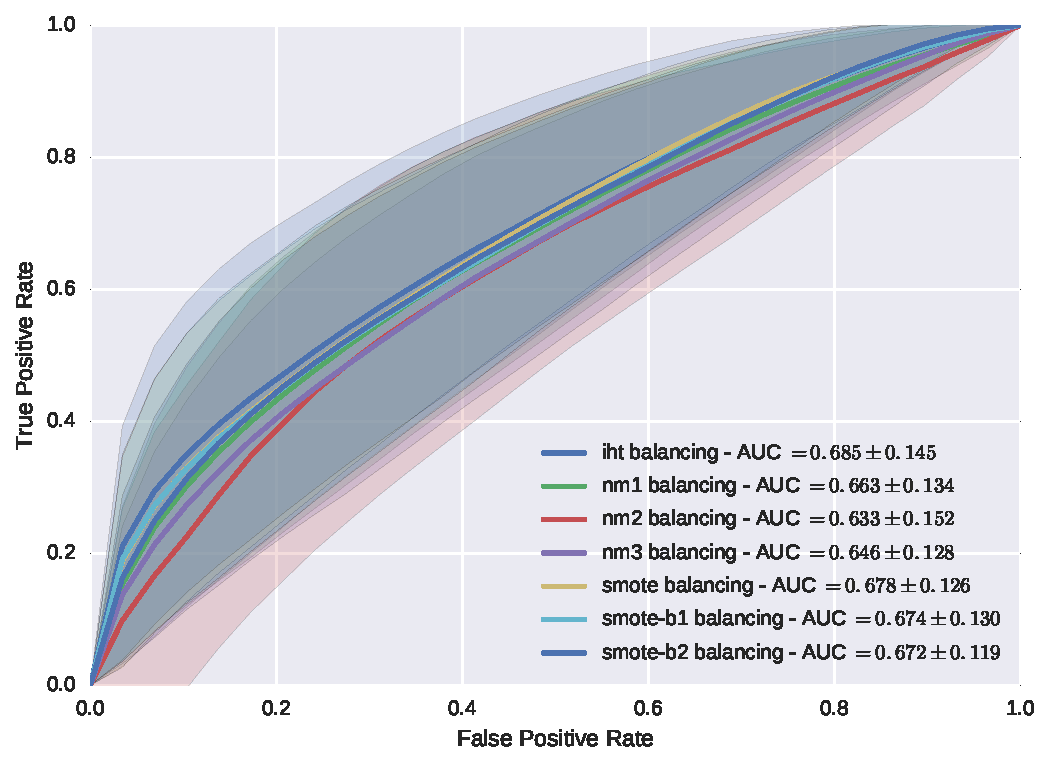
\includegraphics[height=.4\textheight]{6_pipeline/figures/exp-3/dce.pdf}}
  \hfill
  \subfigure[\ac{mrsi}-\ac{mri}]{\label{fig:ex3-MRSI}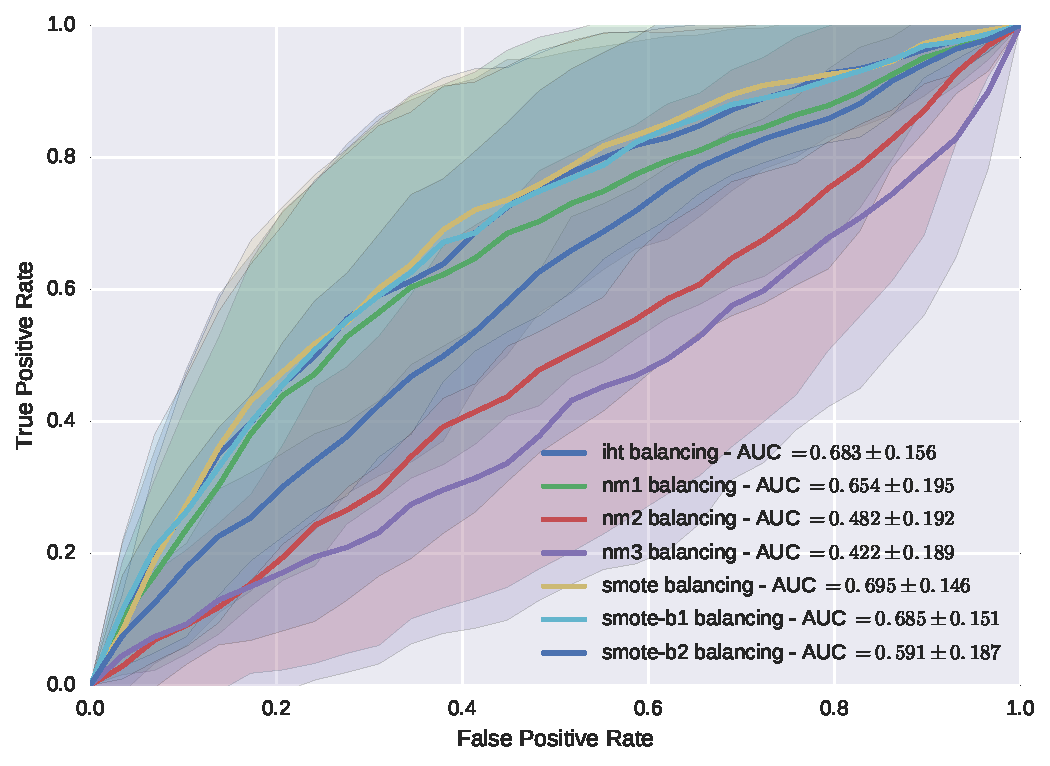
\includegraphics[height=.4\textheight]{6_pipeline/figures/exp-3/mrsi.pdf}}
  \hspace*{\fill}
  \caption{Analysis of the benefit of balancing the training dataset before learning process for each modality.}
  \label{fig:res-Ex3-bal}
\end{figure}

\begin{table}
  \caption{Results in terms of \acs*{auc} of the feature selection based on \acs*{anova} F-value for \acs*{t2w}-\acs*{mri}.}
  \centering
  \scriptsize
  \begin{tabularx}{\linewidth}{@{}l >{\centering\arraybackslash}X >{\centering\arraybackslash}X >{\centering\arraybackslash}X >{\centering\arraybackslash}X >{\centering\arraybackslash}X >{\centering\arraybackslash}X >{\centering\arraybackslash}X @{}}
    \toprule
    \multirow{2}{*}{\textbf{Methods}} & \multicolumn{7}{c}{\textbf{Percentiles}} \\
    \cmidrule{2-8}
    & 15 & 17.5 & 20 & 22.5 & 25 & 27.5 & 30 \\
    \midrule
    \acs*{anova} F-score & $0.755 \pm 0.049$ & $0.770 \pm 0.058$ & $0.777 \pm 0.064$ & $0.782 \pm 0.066$ & $\mathbf{0.784 \pm 0.067}$ & $0.783 \pm 0.072$ & $0.782 \pm 0.070$ \\
    \bottomrule
  \end{tabularx}
  \label{tab:ginit2w}
\end{table}

\begin{table}
  \caption{Results in terms of \acs*{auc} of the feature selection based on Gini importance for \acs*{t2w}-\acs*{mri}.}
  \centering
  \scriptsize
  \begin{tabularx}{\linewidth}{@{}l >{\centering\arraybackslash}X >{\centering\arraybackslash}X >{\centering\arraybackslash}X >{\centering\arraybackslash}X >{\centering\arraybackslash}X >{\centering\arraybackslash}X >{\centering\arraybackslash}X @{}}
    \toprule
    \multirow{2}{*}{\textbf{Methods}} & \multicolumn{7}{c}{\textbf{Percentiles}} \\
    \cmidrule{2-8}
    & 1 & 2 & 5 & 10 & 15 & 20 & 30 \\
    \midrule
    Gini importance & $0.726 \pm 0.064$ & $0.731 \pm 0.055$ & $0.751 \pm 0.065$ & $0.758 \pm 0.076$ & $0.752 \pm 0.087$ & $0.761 \pm 0.077$ & $\mathbf{0.764 \pm 0.079}$ \\
    \bottomrule
  \end{tabularx}
  \label{tab:anovat2w}
\end{table}

\begin{table}
  \caption{Results in terms of \acs*{auc} of the feature selection based on \acs*{anova} F-value for \acs*{adc}.}
  \centering
  \scriptsize
  \begin{tabularx}{\linewidth}{@{}l >{\centering\arraybackslash}X >{\centering\arraybackslash}X >{\centering\arraybackslash}X >{\centering\arraybackslash}X >{\centering\arraybackslash}X >{\centering\arraybackslash}X >{\centering\arraybackslash}X @{}}
    \toprule
    \multirow{2}{*}{\textbf{Methods}} & \multicolumn{7}{c}{\textbf{Percentiles}} \\
    \cmidrule{2-8}
    & 10 & 12.5 & 15 & 17.5 & 20 & 22.5 & 25 \\
    \midrule
    \acs*{anova} F-score & $0.684 \pm 0.123$ & $0.713 \pm 0.125$ & $0.712 \pm 0.134$ & $0.710 \pm 0.144$ & $\mathbf{0.714 \pm 0.142}$ & $0.708 \pm 0.150$ & $0.708 \pm 0.150$ \\
    \bottomrule
  \end{tabularx}
  \label{tab:giniadc}
\end{table}

\begin{table}
  \caption{Results in terms of \acs*{auc} of the feature selection based on Gini importance for \acs*{adc} map.}
  \centering
  \scriptsize
  \begin{tabularx}{\linewidth}{@{}l >{\centering\arraybackslash}X >{\centering\arraybackslash}X >{\centering\arraybackslash}X >{\centering\arraybackslash}X >{\centering\arraybackslash}X >{\centering\arraybackslash}X >{\centering\arraybackslash}X @{}}
    \toprule
    \multirow{2}{*}{\textbf{Methods}} & \multicolumn{7}{c}{\textbf{Percentiles}} \\
    \cmidrule{2-8}
    & 1 & 2 & 5 & 10 & 15 & 20 & 30 \\
    \midrule
    Gini importance & $0.672 \pm 0.132$ & $0.690 \pm 0.138$ & $\mathbf{0.743 \pm 0.139}$ & $0.730 \pm 0.136$ & $0.730 \pm 0.142$ & $0.724 \pm 0.141$ & $0.722 \pm 0.142$ \\
    \bottomrule
  \end{tabularx}
  \label{tab:anovaadc}
\end{table}

\begin{table}
  \caption{Results in terms of \acs*{auc} of the feature extraction methods for \acs*{dce}-\ac{mri}.}
  \centering
  \scriptsize
  \begin{tabularx}{\linewidth}{@{}l >{\centering\arraybackslash}X >{\centering\arraybackslash}X >{\centering\arraybackslash}X >{\centering\arraybackslash}X >{\centering\arraybackslash}X >{\centering\arraybackslash}X >{\centering\arraybackslash}X @{}}
    \toprule
    \multirow{2}{*}{\textbf{Methods}} & \multicolumn{7}{c}{\textbf{Number of components or sparsity level}} \\
    \cmidrule{2-8}
    & 2 & 4 & 8 & 16 & 24 & 32 & 36 \\
    \midrule
    \acs*{pca} & $0.656 \pm 0.133$ & $0.634 \pm 0.121$ & $0.668 \pm 0.149$ & $0.680 \pm 0.145$ & $0.682 \pm 0.146$ & $0.679 \pm 0.151$ & $0.683 \pm 0.149$ \\
    Sparse-\acs*{pca} & $0.578 \pm 0.117$ & $0.546 \pm 0.121$ & $0.554 \pm 0.097$ & --- & --- & --- & --- \\
    \acs*{ica} & $0.657 \pm 0.132$ & $0.629 \pm 0.117$ & $0.671 \pm 0.157$ & $0.686 \pm 0.158$ & $\mathbf{0.691 \pm 0.158}$ & $0.681 \pm 0.161$ & $0.679 \pm 0.166$ \\
    \bottomrule
  \end{tabularx}
  \label{tab:dcefeatext}
\end{table}


\begin{table}
  \caption{Results in terms of \acs*{auc} of the feature extraction methods for \acs*{mrsi}.}
  \centering
  \scriptsize
  \begin{tabularx}{\linewidth}{@{}l >{\centering\arraybackslash}X >{\centering\arraybackslash}X >{\centering\arraybackslash}X >{\centering\arraybackslash}X >{\centering\arraybackslash}X >{\centering\arraybackslash}X >{\centering\arraybackslash}X @{}}
    \toprule
    \multirow{2}{*}{\textbf{Methods}} & \multicolumn{7}{c}{\textbf{Number of components or sparsity level}} \\
    \cmidrule{2-8}
    & 2 & 4 & 8 & 16 & 24 & 32 & 36 \\
    \midrule
    \acs*{pca} & $0.566 \pm 0.120$ & $0.575 \pm 0.141$ & $0.648 \pm 0.162$ & $0.662 \pm 0.177$ & $0.659 \pm 0.184$ & $0.671 \pm 0.179$ & $0.672 \pm 0.182$ \\
    Sparse-\acs*{pca} & $0.502 \pm 0.050$ & $0.571 \pm 0.158$ & $0.585 \pm 0.111$ & --- & --- & --- & --- \\
    \acs*{ica} & $0.567 \pm 0.119$ & $0.578 \pm 0.140$ & $0.654 \pm 0.145$ & $0.656 \pm 0.167$ & $0.650 \pm 0.187$ & $0.663 \pm 0.174$ & $\mathbf{0.677 \pm 0.171}$ \\
    \bottomrule
  \end{tabularx}
  \label{tab:mrsifeatext}
\end{table}

\begin{table}
  \caption{Results in terms of \acs*{auc} of the feature selection based on \acs*{anova} F-value for the aggregation of feature from all \acs*{mpmri} features.}
  \centering
  \scriptsize
  \begin{tabularx}{\linewidth}{@{}l >{\centering\arraybackslash}X >{\centering\arraybackslash}X >{\centering\arraybackslash}X >{\centering\arraybackslash}X >{\centering\arraybackslash}X >{\centering\arraybackslash}X >{\centering\arraybackslash}X @{}}
    \toprule
    \multirow{2}{*}{\textbf{Methods}} & \multicolumn{7}{c}{\textbf{Percentiles}} \\
    \cmidrule{2-8}
    & 10 & 12.5 & 15 & 17.5 & 20 & 22.5 & 25 \\
    \midrule
    \acs*{anova} F-score & $0.764 \pm 0.095$ & $0.765 \pm 0.079$ & $0.800 \pm 0.083$ & $0.817 \pm 0.089$ & $\mathbf{0.828 \pm 0.084}$ & $0.822 \pm 0.0.084$ & $0.815 \pm 0.086$ \\
    \bottomrule
  \end{tabularx}
  \label{tab:anovacomb}
\end{table}

\begin{table}
  \caption{Results in terms of \acs*{auc} of the feature selection based on Gini importance for the aggregation of feature from all \acs*{mpmri} features.}
  \centering
  \scriptsize
  \begin{tabularx}{\linewidth}{@{}l >{\centering\arraybackslash}X >{\centering\arraybackslash}X >{\centering\arraybackslash}X >{\centering\arraybackslash}X >{\centering\arraybackslash}X >{\centering\arraybackslash}X >{\centering\arraybackslash}X @{}}
    \toprule
    \multirow{2}{*}{\textbf{Methods}} & \multicolumn{7}{c}{\textbf{Percentiles}} \\
    \cmidrule{2-8}
    & 10 & 12.5 & 15 & 17.5 & 20 & 22.5 & 25 \\
    \midrule
    Gini importance & $0.834 \pm 0.085$ & $0.834 \pm 0.088$ & $0.834 \pm 0.084$ & $\mathbf{0.836 \pm 0.083}$ & $0.834 \pm 0.079$ & $0.828 \pm 0.086$ & $0.830 \pm 0.077$ \\
    \bottomrule
  \end{tabularx}
  \label{tab:ginicomb}
\end{table}

\begin{table}
  \caption{Selected feature and number of occurrence for \acs*{t2w}-\acs*{mri}, \acs*{adc} map, and one all the features are concatenated.}
  \centering
  \scriptsize
  \begin{tabular}{llllll}
    \toprule
    \multicolumn{1}{c}{\textbf{\acs*{t2w}-\acs*{mri}}} & \multicolumn{1}{c}{\textbf{\acs*{adc}}} & \multicolumn{1}{c}{\textbf{\acs*{t2w}-\acs*{mri}}} & \multicolumn{1}{c}{\textbf{\acs*{adc}}} & \multicolumn{1}{c}{\textbf{\acs*{dce}-\acs*{mri}}} & \multicolumn{1}{c}{\textbf{\acs*{mrsi}}} \\
    \cmidrule(lr){1-1} \cmidrule(lr){2-2} \cmidrule(lr){3-6}
    8 edges & 1 \acs*{dct} & 113 Gabor filters & 53 Gabor filters & 14 samples  & 78 samples \\
    155 Gabor filters & 32 Gabor filters & 1 phase congruency & 2 phase congruency & & \\ 
    2 Haralick features & 1 phase congruency & 4 edges & & & \\
    1 intensity & & 1 intensity & & & \\
    4 \acs*{lbp} & & & & & \\
    2 phase congruency & & & & & \\
    \cmidrule(lr){1-1} \cmidrule(lr){2-2} \cmidrule(lr){3-6}
    \multicolumn{1}{c}{\textbf{172 features}} & \multicolumn{1}{c}{\textbf{34 features}} & \multicolumn{4}{c}{\textbf{267 features}} \\
    \bottomrule
  \end{tabular}
  \label{tab:selfeatocc}
\end{table}

\end{landscape}

% feature selection
% results
In overall, feature selection or extraction lead to increase the classification performance.
For features extracted from the \ac{t2w}\ac{mri}, \ac{anova}-based selection lead to better performance than Gini importance selection, with a \ac{auc} of $0.784 \pm 0.067$.
The opposite conclusion is drawn for the features extracted from the \ac{adc} map.
The selection using the Gini importance criterion leads to an \ac{auc} of $0.743 \pm 0.139$.
% improvements
Therefore, the feature selection leads to an improve \ac{auc} of $0.022$ and $0.013$ for \ac{t2w}-\ac{mri} and \ac{adc} map, respectively.
% which features are selected
The features which have been selected are reported in the 1\textsuperscript{st} and 2\textsuperscript{nd} columns of \acs{tab}~\ref{tab:selfeatocc}.
To conclude, from the 690 original features, 172 and 43 features are selected from the \ac{t2w}-\ac{mri} and \ac{adc} map, respectively.

% feature extraction
Regarding feature extraction, \ac{ica} outperforms other methods for both \ac{mrsi} and \ac{dce}-\ac{mri} with \ac{auc} scores of $0.677 \pm 0.171$ and $0.691 \pm 0.158$, respectively.
However, only the projection applied to \ac{dce}-\ac{mri} features leads to improved results with a gain of $0.013$ with 24 components selected instead of the original 40 dimensions.

% feature selection for concatenation
% results
Gini importance selection method is also outperforming \ac{anova}-based method while selecting the features from the concatenation of all of them.
The reported \ac{auc} is $0.836 \pm 0.083$ with an increase of $0.034$.
% which features are selected
The features which have been selected are reported from the 3\textsuperscript{rd} to the 6\textsuperscript{th} columns of \acs{tab}~\ref{tab:selfeatocc}.
To conclude, from the 1533 original features, 267 features are selected from the entire set of feature.

\subsection{Fine-tuned combination of \ac{mpmri} modalities}\label{subsec:chp6:exp-res:Ex4}

\begin{figure}
  \centering
  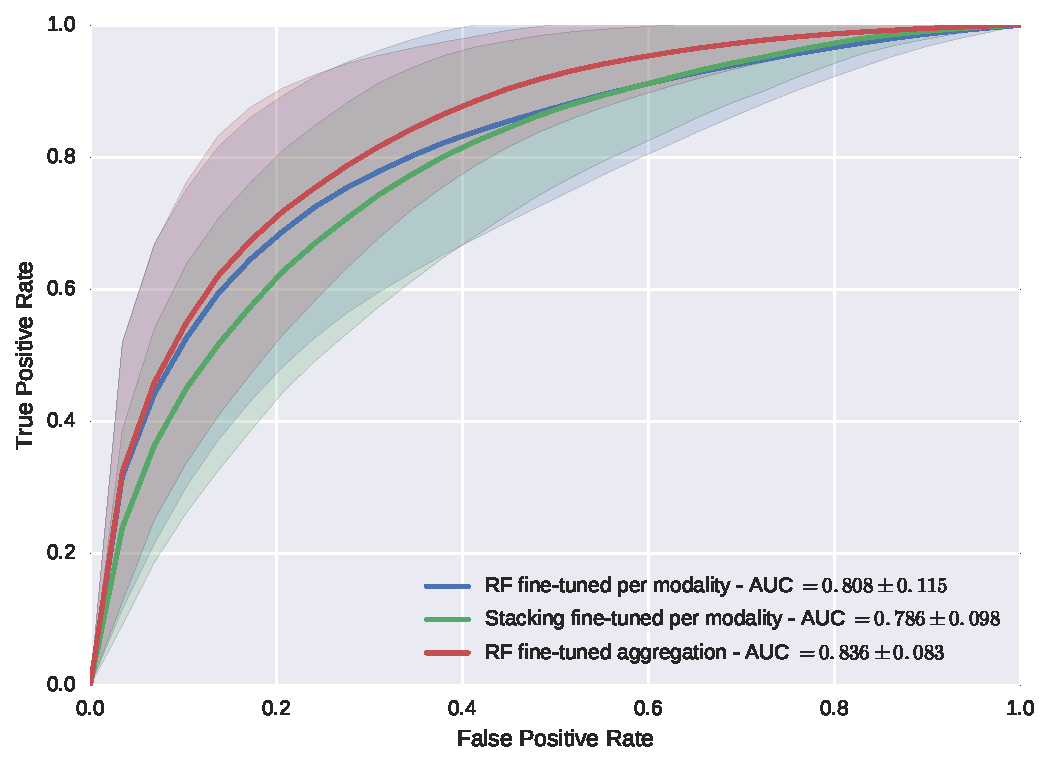
\includegraphics[width=0.7\linewidth]{6_pipeline/figures/exp-5/combine_all.pdf}
  \caption[Analysis of feature combination approaches after fine tuning.]{Analysis of feature combination approaches after fine tuning through balancing and feature selection/extraction.}
  \label{fig:res-Ex4}
\end{figure}

\begin{figure}
  \centering
  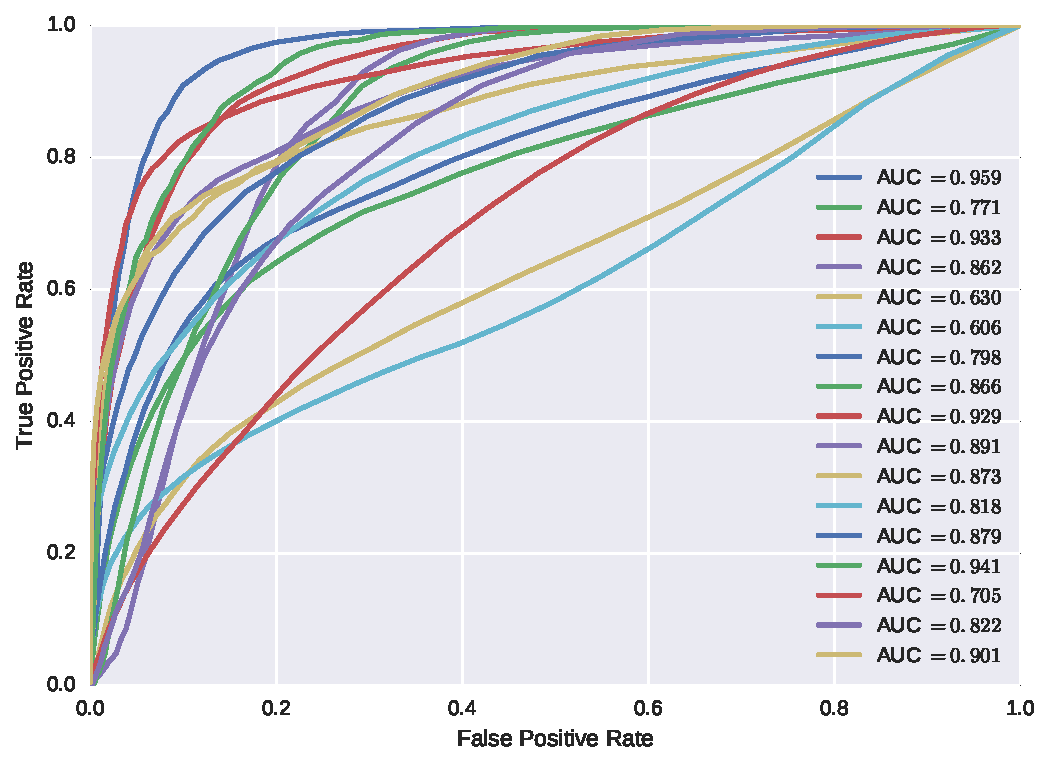
\includegraphics[width=0.7\linewidth]{6_pipeline/figures/exp-5/plot_all_patients.pdf}
  \caption{Individual patient \acs*{auc} for the best configuration of the \acs*{mpmri} \acs*{cad}.}
  \label{fig:indauc}
\end{figure}

This experiment aims at providing the most efficient \ac{mpmri} \ac{cad} for \ac{cap} using the fine-tuned feature space from the previous experiment.
Three strategies are applied:
(i) the selected features from each modality --- i.e., 331 features --- are concatenated together and used in a \ac{rf} classifier,
(ii) the selected features from each modality --- i.e., 331 features --- are used to train a stacking classifier with a \ac{gb} as meta-classifier, and
(iii) the selected features from the concatenated set of feature --- i.e., 267 features --- are used to train a single \ac{rf} classifier.

\begin{landscape}
\begin{figure}
  \hspace*{\fill}
  \subfigure[\acs*{auc} = 0.922]{\label{fig:pat634}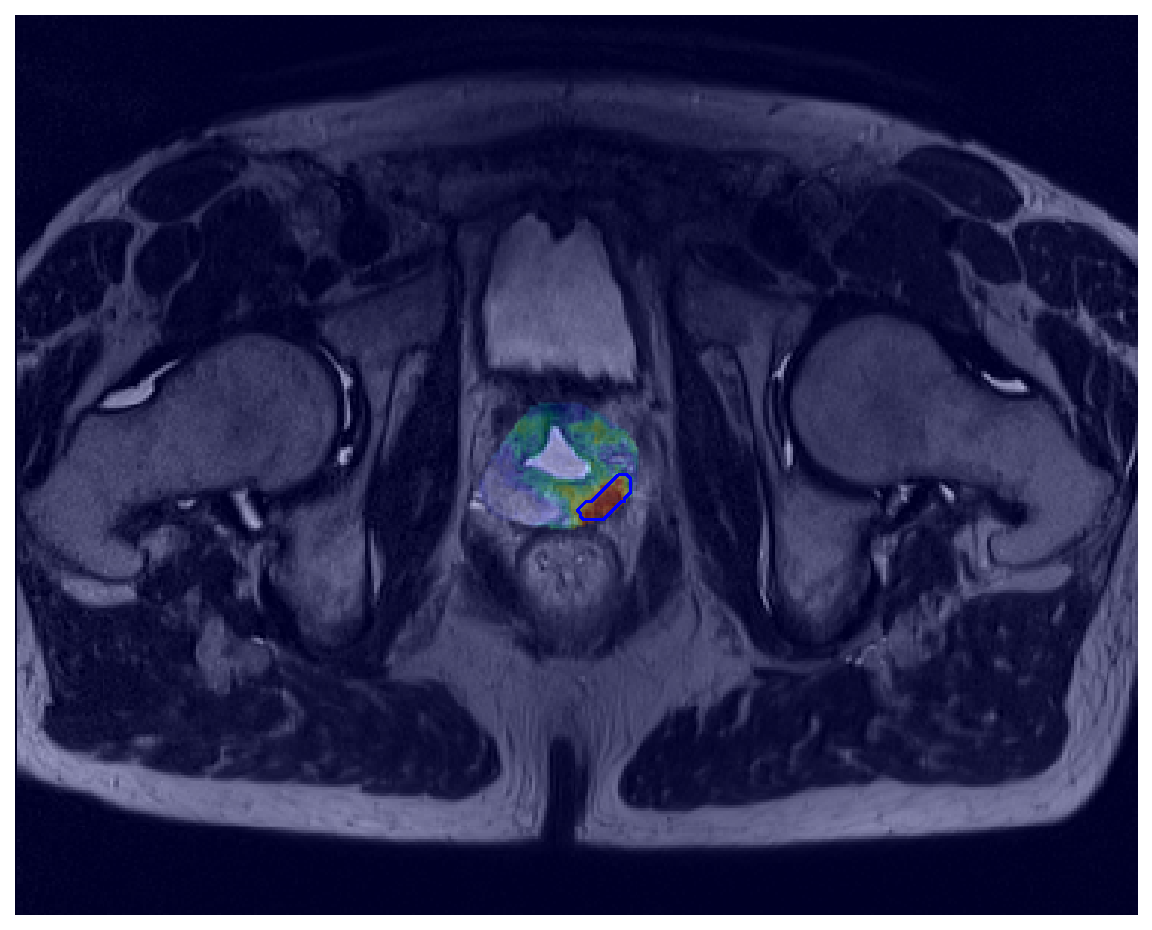
\includegraphics[width=.45\textwidth]{6_pipeline/figures/examples/patient_634.pdf}}
  \hfill
  \subfigure[\acs*{auc} = 0.942]{\label{fig:pat778}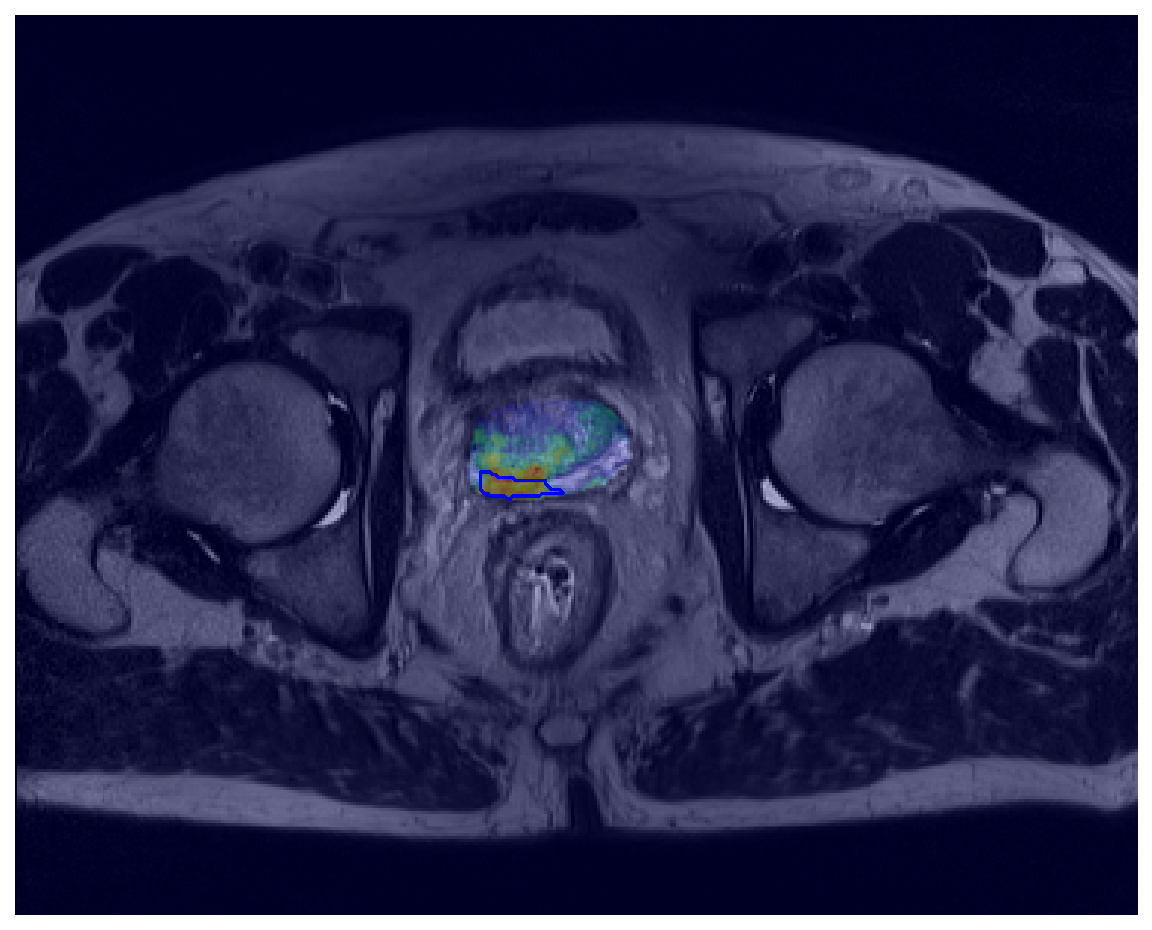
\includegraphics[width=.45\textwidth]{6_pipeline/figures/examples/patient_778.pdf}}
  \hfill
  \subfigure[\acs*{auc} = 0.914]{\label{fig:pat1036}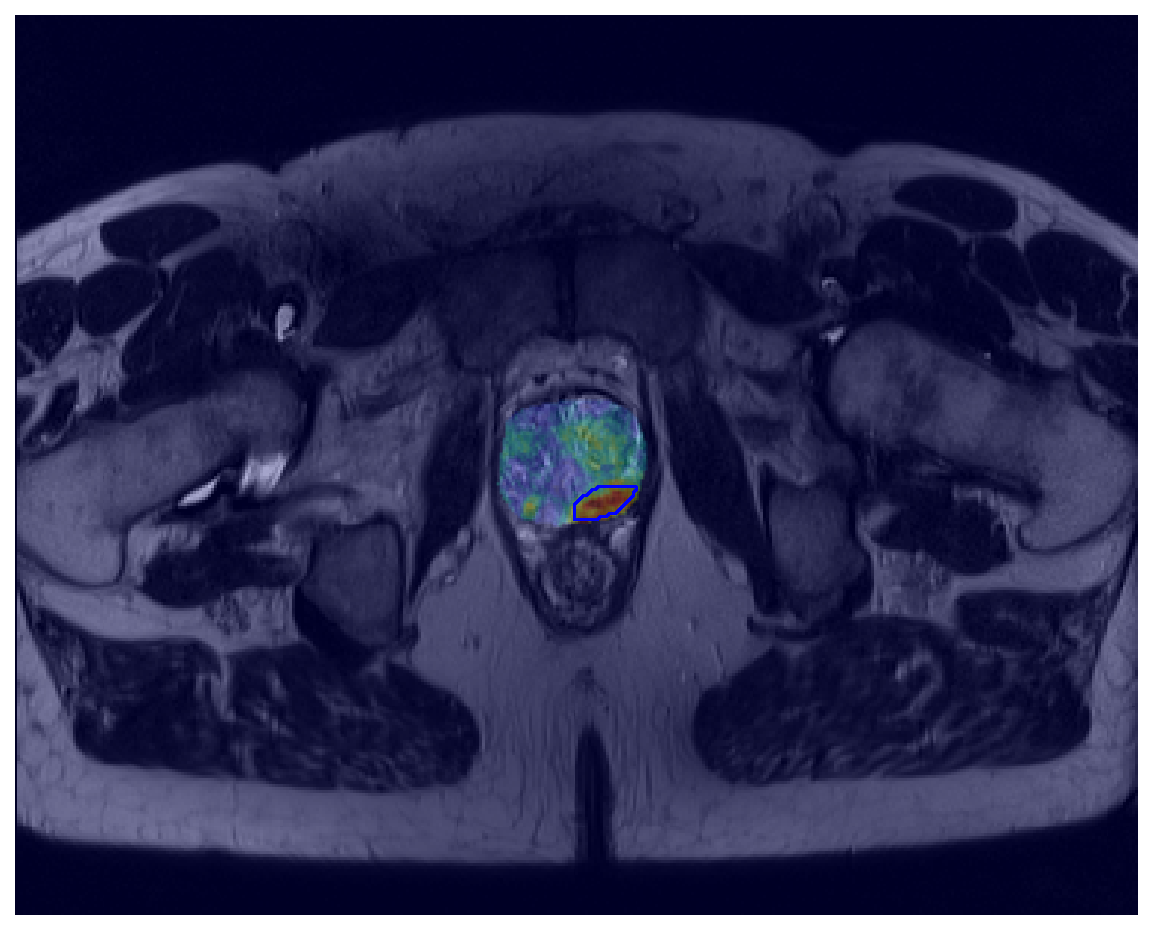
\includegraphics[width=.45\textwidth]{6_pipeline/figures/examples/patient_1036.pdf}}
  \hspace*{\fill}\\
  \hspace*{\fill}
  \subfigure[\acs*{auc} = 0.692]{\label{fig:pat634}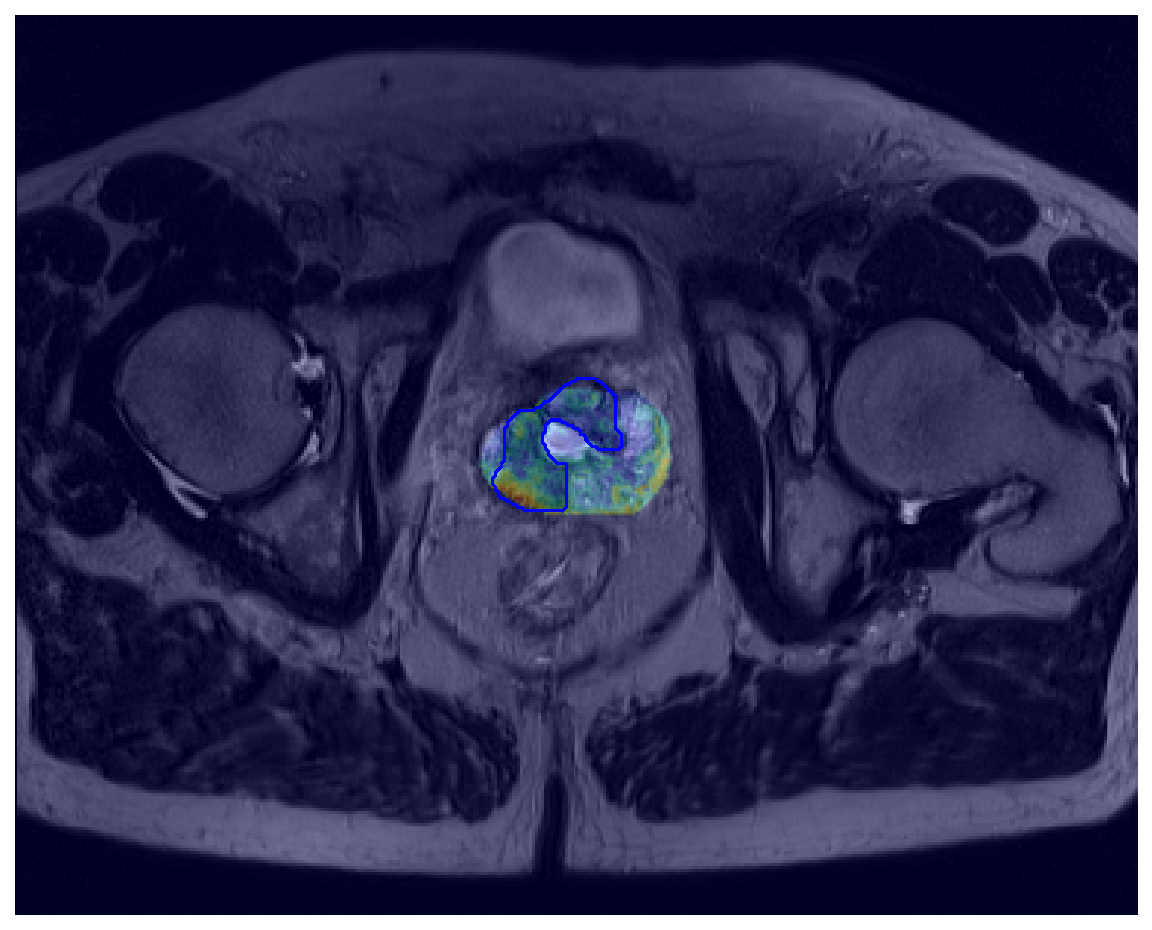
\includegraphics[width=.45\textwidth]{6_pipeline/figures/examples/patient_410.pdf}}
  \hfill
  \subfigure[\acs*{auc} = 0.879]{\label{fig:pat778}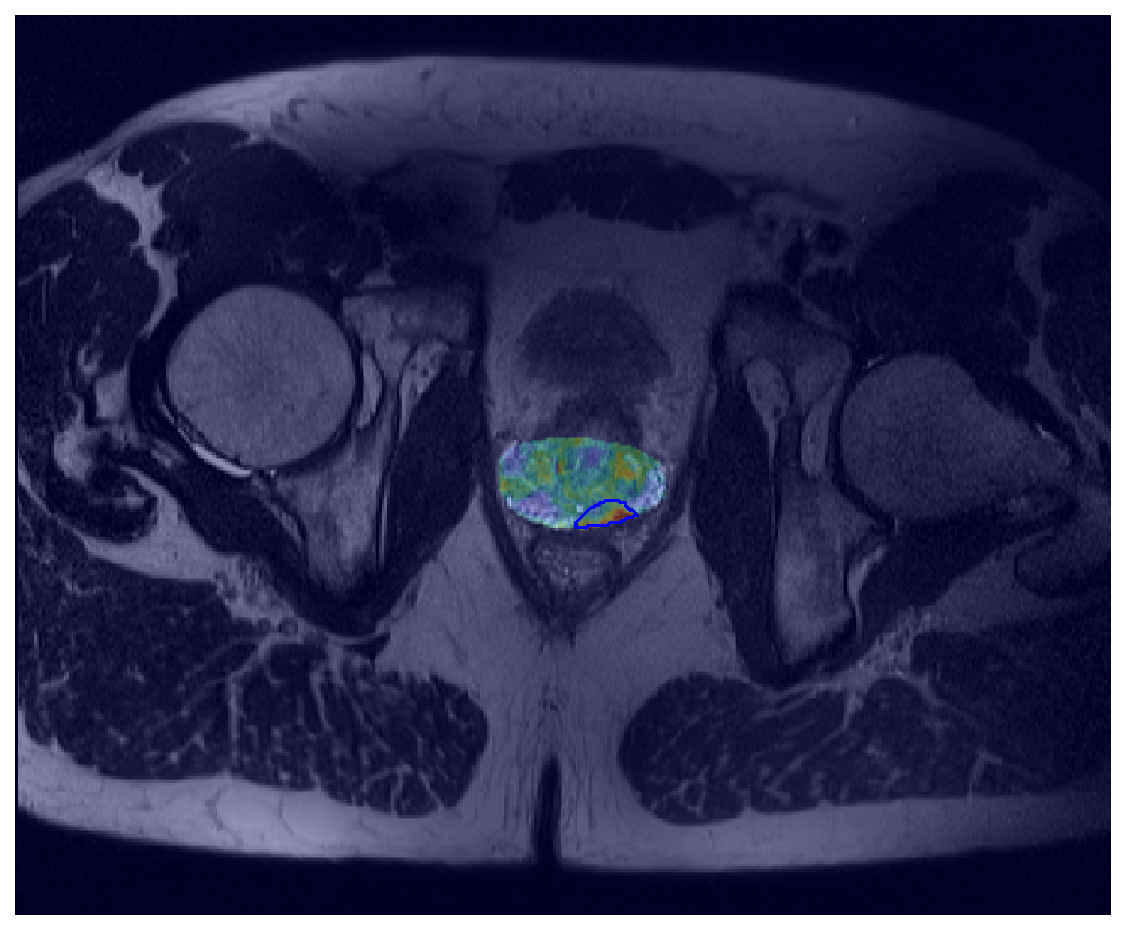
\includegraphics[width=.45\textwidth]{6_pipeline/figures/examples/patient_784.pdf}}
  \hfill
  \subfigure[\acs*{auc} = 0.735]{\label{fig:pat1036}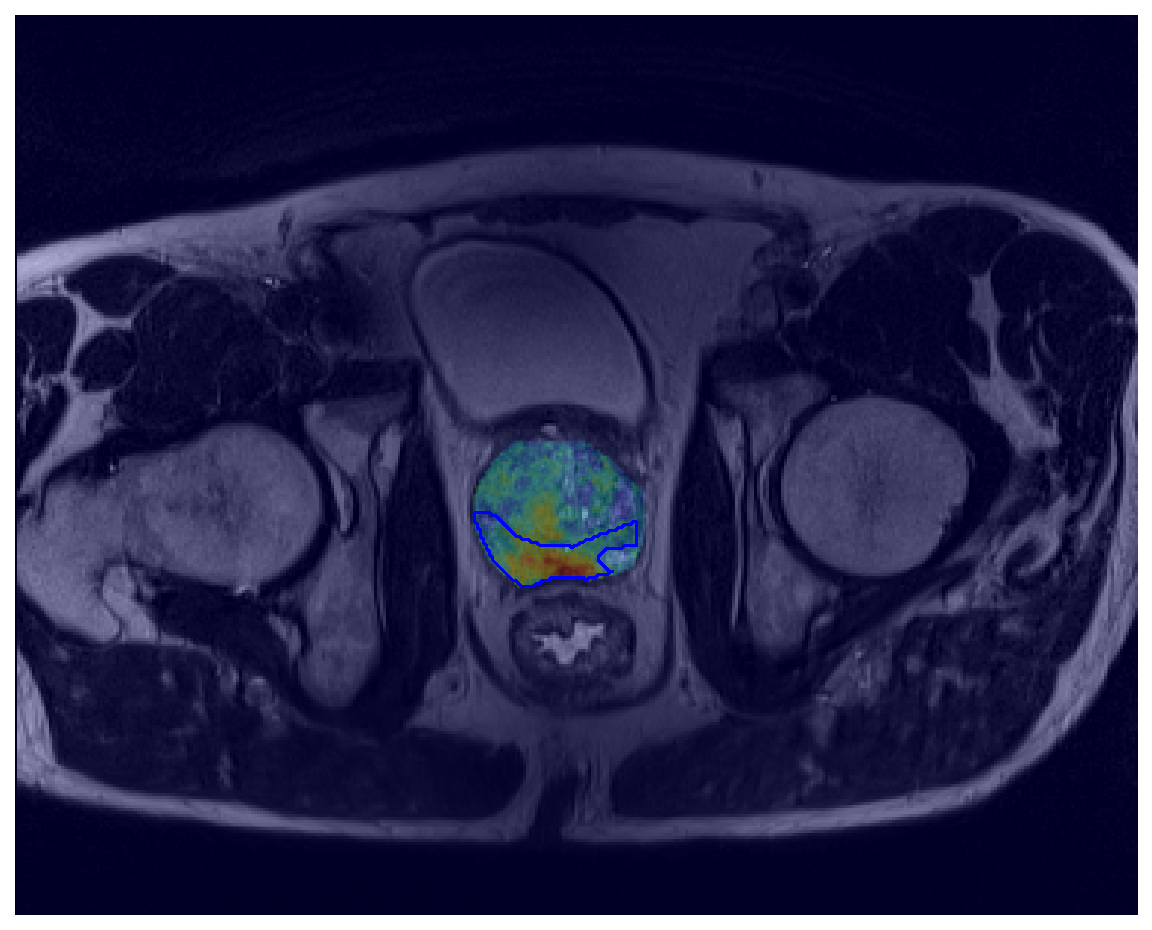
\includegraphics[width=.45\textwidth]{6_pipeline/figures/examples/patient_1041.pdf}}
  \hspace*{\fill}
  \caption[Illustration the resulting detection of our \acs*{mpmri} \acs*{cad} for \acs*{cap} detection.]{Illustration the resulting detection of our \acs*{mpmri} \acs*{cad} for \acs*{cap} detection. The blue contours corresponds to the \ac{cap} while the \texttt{jet} overlay represents the probability.}
  \label{fig:resultcad}
\end{figure}
\end{landscape}

As previously done, the experiment is performed in a \ac{lopo} fashion and a \ac{roc} analysis is carried out.
The comparative results are shown in \acs{fig}\,\ref{fig:res-Ex4}.
In overall, classification using the fine-tuned features improve the classification performance.
The third classification configuration is, however, the one which outperforms others with an \ac{auc} of $0.836 \pm 0.083$.
The improvement in terms of \ac{auc} is of $0.028$ and $0.050$ compared with the 1\textsuperscript{st} and 2\textsuperscript{nd}, respectively.

Additionally, the individual \ac{roc} analysis for each patient for the best configuration is shown in \acs{fig}\,\ref{fig:indauc}.
It can be noted that 12 patients have an \ac{auc} superior to $0.800$ and 2 patients have a rather low \ac{auc} below $0.700$.
Regarding the 4 patients with an \ac{auc} below $0.800$, 3 patients have a \ac{cap} localized in the \ac{cg}.

To illustrate qualitatively the results of our \ac{mpmri} \ac{cad} system, 6 diverse examples are presented in \acs{fig}\,\ref{fig:resultcad} by overlapping the probability map of having a \ac{cap} with the original \ac{t2w}-\ac{mri} slice.

\subsection{Benefit of the \acs*{mrsi} modality}\label{subsec:chp6:exp-res:Ex5}

\begin{figure}
  \centering
  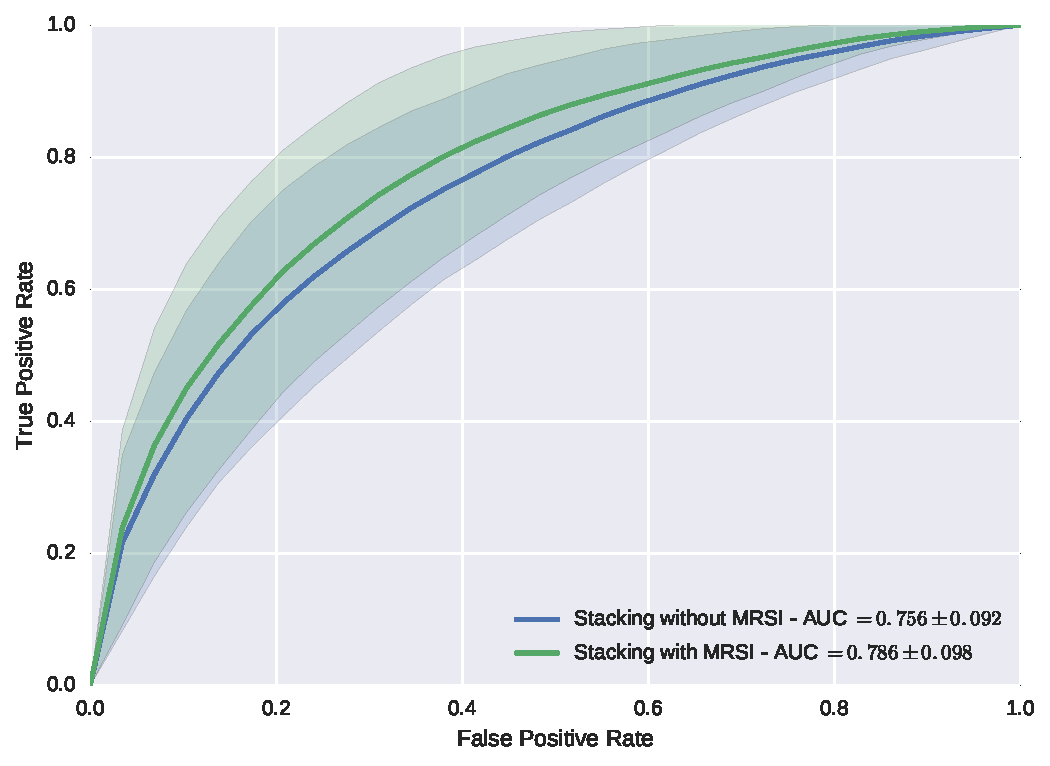
\includegraphics[width=0.7\linewidth]{6_pipeline/figures/exp-6/stacking_wt_mrsi.pdf}
  \caption{Illustration of the gain of including the \acs*{mrsi} modality in a \acs*{mpmri} \acs*{cad}.}
  \label{fig:resmrsigain}
\end{figure}

We recall that the goal of this thesis is to use all the \ac{mpmri} modalities.
In this regard, \ac{mrsi} has nearly never been used together with the other modalities --- i.e., \ac{t2w}-\ac{mri}, \ac{dce}-\ac{mri}, and \ac{adc} map --- apart of the recent work of \citeauthor{trigui2017automatic}~\cite{trigui2016classification,trigui2017automatic}.
Therefore, we propose in this experiment to compare the classification performance by removing the \ac{mrsi} feature.
In this regard, we propose to train 2 stacking classifiers --- with a \ac{gb} as meta-classifier --- while removing the feature related to \ac{mrsi} for one of them.
The same \ac{lopo} validation model is used as before and the results obtained from \ac{roc} analysis are depicted in \acs{fig}\,\ref{fig:resmrsigain}.

Therefore, including \ac{mrsi} into the classification pipeline increases the \ac{auc} from $0.756 \pm 0.092$ to $0.786 \pm 0.098$ for a gain of $0.030$.
